\begin{table*}[t]
\centering\begin{minipage}{\textwidth}
\refstepcounter{table}\label{tab:components}
{\fontsize{9.3}{12}\selectfont\textbf{Table~\thetable.} Frozen follow-up held accuracy (\%). Corrupted conditions average all five mask realizations within each training seed; cells show mean $\pm$ sample SD across five training seeds after pooling the three held sets. R50/B50 use linear repair. All four MIRA configurations have 40,871 nominal trainable parameters; both residual controls have 511,111.\par}
\vspace{5pt}\begingroup\sffamily\fontsize{9.2}{12}\selectfont
\setlength{\tabcolsep}{6pt}\renewcommand{\arraystretch}{1.5}
\begin{tabularx}{\linewidth}{>{\raggedright\arraybackslash}p{.34\linewidth}*{3}{>{\centering\arraybackslash}X}}
\rowcolor{foresthead}\multicolumn{1}{l}{\textcolor{white}{\bfseries Configuration}} & \multicolumn{1}{c}{\textcolor{white}{\bfseries Complete}} & \multicolumn{1}{c}{\textcolor{white}{\bfseries R50}} & \multicolumn{1}{c}{\textcolor{white}{\bfseries B50}}\\
\rowcolor{mintfill}MIRA full reference & $23.73\pm2.26$ & $22.68\pm2.03$ & $22.56\pm1.28$\\
\rowcolor{referencefill}Zero explicit mask input & $23.41\pm1.03$ & $23.22\pm1.23$ & $21.90\pm0.53$\\
\rowcolor{mintfill}Zero distance input & $24.03\pm1.87$ & $22.85\pm1.87$ & $22.77\pm1.02$\\
\rowcolor{referencefill}Uniform temporal pooling & $24.17\pm2.54$ & $23.22\pm1.86$ & $21.30\pm1.57$\\
\rowcolor{lossfill}Residual CNN, clean training & $33.83\pm0.82$ & $33.33\pm0.87$ & $26.72\pm0.67$\\
\rowcolor{shiftfill}Residual CNN, augmented & $30.25\pm1.65$ & $30.09\pm1.70$ & $25.72\pm1.35$\\
\end{tabularx}\endgroup\end{minipage}\end{table*}

\begin{figure*}[t]
\centering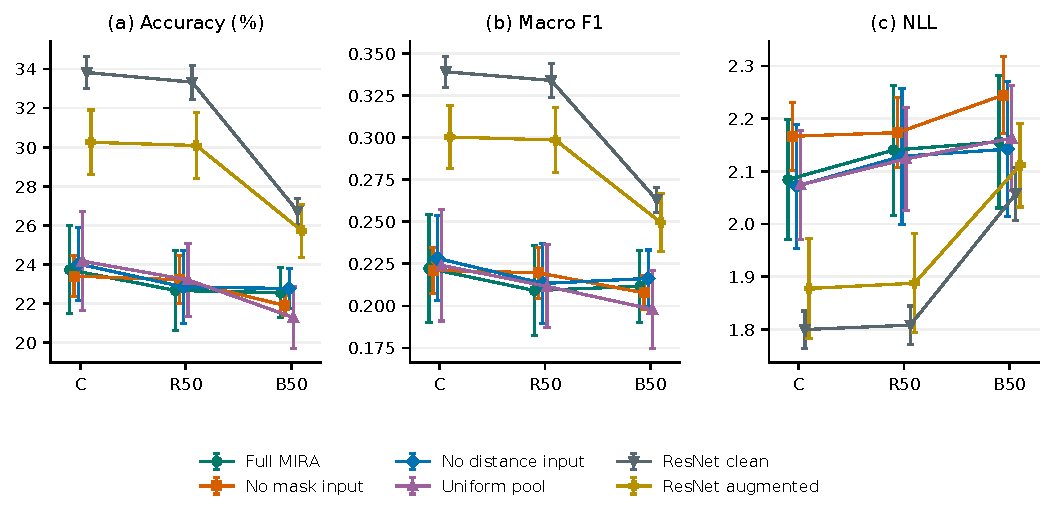
\includegraphics[width=\textwidth]{component_model_comparison.pdf}
\caption{Frozen follow-up comparison of accuracy, macro F1 and source-temperature-calibrated NLL. C is complete input; R50/B50 are random/contiguous 50\% loss with linear repair. Metrics pool 1,260 held files within each training/mask cell, then average masks within training seed. Points show means and bars sample SD across five training seeds on fixed recordings and partitions; they are not confidence intervals for new environments. Higher accuracy/F1 and lower NLL are preferred.}
\label{fig:componentmodels}
\end{figure*}

The larger residual clean-training control reaches 33.83\% held accuracy on complete input and 26.72\% under block loss (Table~\ref{tab:components}, Figure~\ref{fig:componentmodels}); its augmented counterpart reaches 30.25\% and 25.72\%. The residual architectures improve these particular compact-network results, but changing architecture and capacity together does not identify the cause of that difference or establish a generally optimal model. The full MIRA reference reproduces its original clean accuracy. Its block value here averages the full mask grid and therefore differs from the earlier five paired-mask summary. SD across these five mask-averaged seed summaries is not the same quantity as SD across the original five diagonal training/mask pairs. For conditionally independent, identically distributed mask draws within a fixed fit, averaging five masks reduces that fit's mask-variance component by a factor of five; this is not a rule for the total variability across trained models.

For component contrasts, 10,000 paired participant-cluster bootstrap draws sample ten participants with replacement within each fixed environment and retain their complete seed/mask grid. The full model minus each of the three removal controls under linear B50 defines one three-comparison macro-F1 family. Table~\ref{tab:componentcontrasts} reports ordinary 95\% percentile ranges and Bonferroni-adjusted 98.333\% marginal percentile ranges for that family. These approximate conditional sensitivity ranges remain exploratory, depend on within-environment participant exchangeability and fixed fitted models, and do not cover new rooms, retraining or all secondary outcomes. The resampling unit is the participant rather than an individual mask view.

\begin{table*}[t]
\centering\begin{minipage}{\textwidth}
\refstepcounter{table}\label{tab:componentcontrasts}
{\fontsize{9.3}{12}\selectfont\textbf{Table~\thetable.} Component contrasts under contiguous 50\% loss with linear repair. Differences are full MIRA minus the named control in pooled macro F1. The second column adds sample SD of paired, mask-averaged differences across five training seeds; the final column counts positive seed differences. Percentile ranges share identical participant draws, condition on the fixed fitted models, and address only the three contrasts shown.\par}
\vspace{5pt}\begingroup\sffamily\fontsize{9.1}{12}\selectfont
\setlength{\tabcolsep}{5pt}\renewcommand{\arraystretch}{1.5}
\begin{tabularx}{\linewidth}{>{\raggedright\arraybackslash}p{.27\linewidth}>{\centering\arraybackslash}p{.17\linewidth}*{2}{>{\centering\arraybackslash}X}>{\centering\arraybackslash}p{.10\linewidth}}
\rowcolor{purplehead}\multicolumn{1}{l}{\textcolor{white}{\bfseries Control}} & \multicolumn{1}{c}{\textcolor{white}{\bfseries $\Delta$ F1 $\pm$ SD}} & \multicolumn{1}{c}{\textcolor{white}{\bfseries Conditional 95\%}} & \multicolumn{1}{c}{\textcolor{white}{\bfseries Adjusted 98.333\%}} & \multicolumn{1}{c}{\textcolor{white}{\bfseries Positive}}\\
\rowcolor{lavenderfill}Zero explicit mask input & $+0.0039\pm0.0126$ & $[-0.0074,0.0155]$ & $[-0.0096,0.0180]$ & $3/5$\\
\rowcolor{lavenderlight}Zero distance input & $-0.0047\pm0.0117$ & $[-0.0080,-0.0015]$ & $[-0.0086,-0.0007]$ & $2/5$\\
\rowcolor{lavenderfill}Uniform temporal pooling & $+0.0137\pm0.0190$ & $[0.0001,0.0275]$ & $[-0.0023,0.0302]$ & $4/5$\\
\end{tabularx}\endgroup\end{minipage}\end{table*}

The explicit mask-input contrast is inconclusive in this condition. Omitting the distance input gives a small higher mean macro F1 than the full reference, including under the declared conditional three-contrast adjustment; however, the paired difference changes direction across training seeds (Table~\ref{tab:componentcontrasts}). It is not a stable advantage across every initialization. Coverage weighting has a positive unadjusted range, but its adjusted range includes zero (Figure~\ref{fig:componentfamily}). Thus the experiment does not support presenting all three MIRA components as individually beneficial. These condition-specific findings neither prove that a component has no value elsewhere nor validate the full architecture as superior to the reference transform. Different complete-input scores after channel removal are also compatible with retraining under a different parameterization: even a constant clean mask channel can change convolutional activations and the optimization trajectory, including padding-boundary effects. No physical mechanism is identified by that score difference alone.

\begin{figure*}[t]
\centering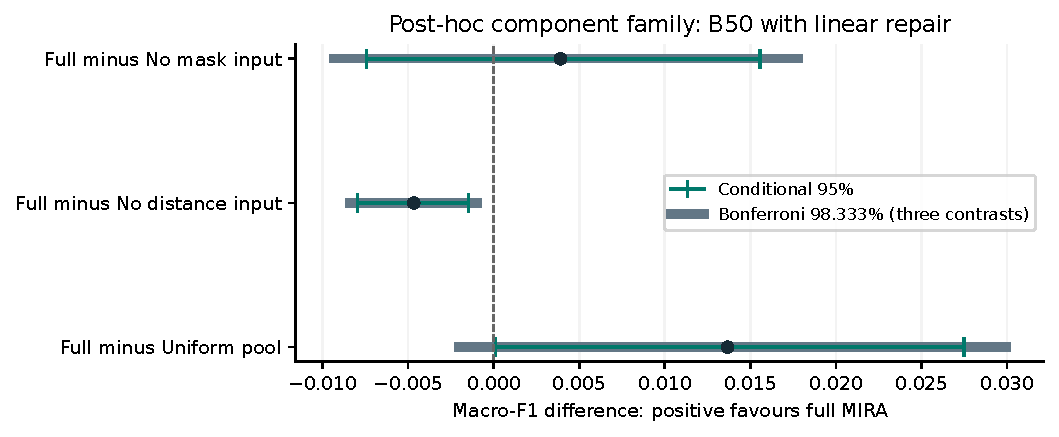
\includegraphics[width=\textwidth]{component_family_intervals.pdf}
\caption{Paired component differences under linear B50. Thin green segments with terminal ticks mark unadjusted 95\% participant-bootstrap percentile ranges; thick gray segments mark 98.333\% ranges adjusted for the three displayed contrasts. Each point is full MIRA minus a removal control, so positive values favour the full model. All ranges use the same 10,000 participant draws within the three fixed environment/cohort strata. This exploratory post-hoc analysis does not measure uncertainty over new environments or model retraining.}
\label{fig:componentfamily}
\end{figure*}
